\documentclass[tikz,border=10pt]{standalone}
\begin{document}
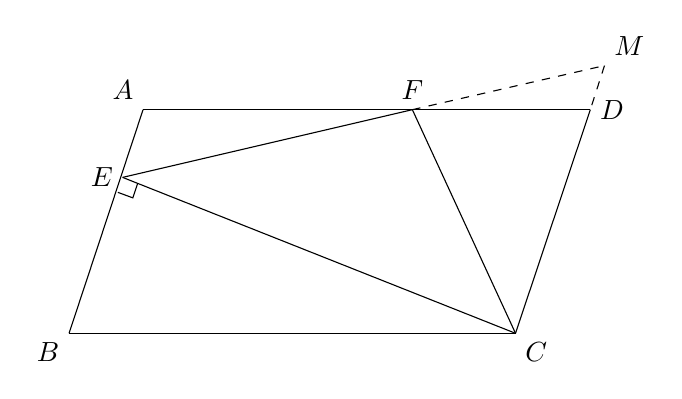
\begin{tikzpicture}
\coordinate (A) at (1.42,2.88);
\coordinate (D) at (7.10,2.88);
\coordinate (B) at (0.48,0.04);
\coordinate (C) at (6.15,0.04);
\coordinate (E) at (1.16,2.02);
\coordinate (F) at (4.84,2.88);
\coordinate (M) at (7.28,3.44);
\coordinate (R1) at (1.10,1.83);
\coordinate (R2) at (1.29,1.76);
\coordinate (R3) at (1.35,1.94);

\draw (A) -- (D);
\draw (A) -- (B);
\draw (B) -- (C);
\draw (C) -- (D);
\draw (E) -- (F);
\draw (E) -- (C);
\draw (F) -- (C);
\draw[dashed] (F) -- (M);
\draw[dashed] (M) -- (D);
\draw (R1) -- (R2) -- (R3);

\node[above left] at (A) {$A$};
\node[above] at (F) {$F$};
\node[right] at (D) {$D$};
\node[above right] at (M) {$M$};
\node[left] at (E) {$E$};
\node[below left] at (B) {$B$};
\node[below right] at (C) {$C$};
\end{tikzpicture}
\end{document}
